\hypertarget{power-estimation}{%
\chapter{Power Estimation}\label{power-estimation}}

In this tutorial we will learn how to estimate the power by using
ModelSim to generate the switching activity of the design, and XPower
(from Xilinx) to analyze the results and generate the final power report
and CosmosScope to visualize the results.

\hypertarget{different-types-of-power}{%
\section{Different Types of Power}\label{different-types-of-power}}

Typically, power dissipation in a cell is subdivided into two different
groups, dynamic power, and static power. \textbf{Dynamic power} is the
power dissipated in a cell when the input voltage is actively
transitioning. Dynamic power is further subdivided into two components
switching power and internal power. \textbf{Switching power} is the
power required to charge the capacitive load on the output pins of the
cell. Switching power is shown in Figure \ref{fig:fig71},
as the I\textsubscript{sw} switching current charging up the
C\textsubscript{load} capacitor. This component of power is calculated
using the familiar ½ CV\textsuperscript{2} equation.

For switching power, all we need to know is V\textsubscript{dd} and the
capacitive load that is driven by the cell. Therefore, the library does
not need to be characterized for this component of power dissipation.
\begin{figure}[!htb]
	\centering
	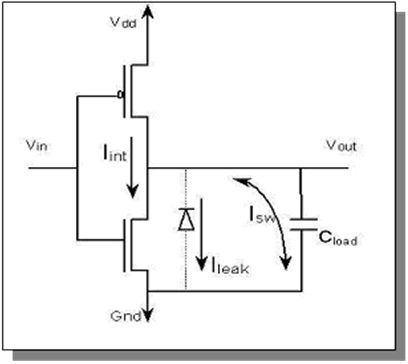
\includegraphics[width=0.7\textwidth]{src/images/7-1.png}
	\caption{Switching Power Dissipation}
	\label{fig:fig71}
\end{figure}
\textbf{Internal power} consists of short-circuit power and power
dissipated by charging the capacitive loads that are internal to the
cell (not shown in the above circuit). Short-circuit power is the power
that is dissipated due to the short period that paths in the cell are
essentially short circuits. In the circuit shown above,
I\textsubscript{int}, that is the current path when the device is
short-circuited, shows internal power. Every time the input
V\textsubscript{in} toggles, there is a short period of time where both
transistors are turned on and there is a path from V\textsubscript{dd}
to ground. The longer both transistors are active, the higher the power
dissipation. The circuit above is quite simple (an inverter) and there
is only one path from V\textsubscript{dd} to ground. For complex
circuits, you could have dozens of potential short circuit paths.
Internal power is dependent on the transition time of the input voltage
V\textsubscript{in} and the output capacitive load. These factors
determine how long the short circuit is active. There is no easy formula
to determine the power dissipated due to internal power, so the cell
must be characterized for it.

\begin{quote}
The final component of power analysis is the \textbf{Leakage power}. In
the circuit diagram in Figure 7-1, it is shown as leak current. This is
the power dissipated when the circuit is in a steady state and it is due
to the following factors inherent in transistors: reverse bias leakage
current, sub-threshold current, or other second-order leakage power.
Leakage power has become a major factor in power analysis in recent era.
\end{quote}

At 180 nm and above, leakage power was typically less than 1\% of the
total power dissipation in a circuit. With 130 nm and below, the leakage
power becomes a much larger factor, up to 50\% of dissipated power in
some cases. Leakage power should be characterized for each cell in the
library.

To report the switching power, we need the switching activities of the
design. The switching activity contains information about the static
probability and toggle rate. The static probability can be calculated
during a simulation by comparing the time a signal is at a certain logic
state (state 0 or state 1) to the total time of simulation. The toggle
rate is the number of transitions between logic-0 and logic-1 (or vice
versa) of a design object per unit of time.

The previous power definitions can be concluded by these two equations:
\begin{lstlisting}
Total Power = Dynamic power + Leakage power
Dynamic Power = Switching power + Internal power	
\end{lstlisting}
\hypertarget{estimating-the-power-consumption}{%
\section{Estimating the Power
Consumption}\label{estimating-the-power-consumption}}

To estimate the power consumption for a specific application on a
specific CPU you need to generate the switching activities, which are
saved as a Value Change Dump (VCD) file. This file is generated when the
project is simulated using ModelSim and the application is executed on
the CPU. Then the VCD file will be used as input to the XPower tool,
which finally will generate the power report. This report can be
visualized using the CosmosScope visualization tool.

\hypertarget{generate-the-vcd-file-using-modelsim}{%
\subsection{Generate the VCD file using
ModelSim}\label{generate-the-vcd-file-using-modelsim}}

The VCD (Value Change Dump) file can be generated during the ModelSim
simulation to capture signals switching activities as explained below:

\begin{enumerate}
\def\labelenumi{(\arabic{enumi})}
\item
  Create a ModelSim project in your project's \emph{ModelSim} directory,
  add your CPU VHDL files from your project's ``\emph{meister/*.syn}''
  directory, and add testbench files from the \emph{ModelSim} directory,
  as explained in the Chapter. Remember that you should already have
  generated \emph{TestData.IM} and \emph{TestData.DM} files in your
  \emph{ModelSim} directory using ``\emph{make sim}''.
\item
  Configure the CPU Frequency for which you want to run the power
  estimation. Open the ModelSim testbench (\emph{tb\_browstd32.vhd}),
  search for CLK\_PERIOD, and change the value accordingly. Take care:
  For simulation-reasons this value corresponds to the time (in
  nanoseconds) of a half clock period. For example, 10 ns half period
  correspond to 20 ns clock period, which is 50 MHz frequency.
\item
  Compile the project Compile Compile Order Auto Generate
\item
  Start the simulation: VSIM \textgreater{} \textbf{vsim -t 1ns
  work.cfg}
\item
  Store the switching activities during the program execution in the VCD
  file e.g. ``\emph{test.vcd}'' by typing: VSIM \textgreater{}
  \textbf{vcd file test.vcd}
\item
  Add all signals of the CPU instance: VSIM \textgreater{} \textbf{vcd
  add -r test/dut/*}
\item
  The entity name of the tutorial example testbench is \emph{test} and
  the instance name of the device under test is \emph{dut}. Using the
  \emph{-r} switch with ModelSim ``\emph{vcd add}'' command will result
  in a large but significantly more accurate VCD file. VCD files can
  grow quite large for larger designs or even for smaller designs if the
  simulation time is long.
\item
  Run the simulation: VSIM \textgreater{} \textbf{run -all}
\item
  The switching activities will be saved in ``test.vcd'' file.
\end{enumerate}

\hypertarget{generating-the-power-report-using-xpower}{%
\subsection{Generating the Power Report Using
xPower}\label{generating-the-power-report-using-xpower}}

The second step is to create an ISE project that you want to analyze for
power consumption. Create a new project and add only the CPU files from
the ASIP Meister ``\emph{meister/xxx.syn}'' directory to it. In the
``\emph{Processes}''-tree of your top-level design and under
``\emph{Implement Design/Place \& Route}'', click on ``\emph{Analyze
Power Distribution (xPower Analyzer)}''. This will open the xPower
window. Now, click on ``\emph{File\textgreater open Design}'', in the
``\emph{Design}'' file, you have to add your .ncd file e.g.
toplevel.ncd'' and in ``\emph{Simulation Activity}'' file, you have to
add the .vcd file that you generated in the previous step. Finally, in
the ``\emph{Physical Constraint}'' file, you can add the .pcf file for
you project e.g. ``toplevel.pcf'' as shown in Figure \ref{fig:fig72}. As soon as you click OK, the
XPower tool will analyze the files and gives you a summary about the
power consumption in your design (like the Leakage power and the total
power). On the right side, you find ``By Clock Domain''. Here you see
the frequency in (MHz). The clock frequency should be the same frequency
that you used in testbench during VCD file generated as shown in Figure \ref{fig:fig73}.
\begin{figure}[!htb]
	\centering
	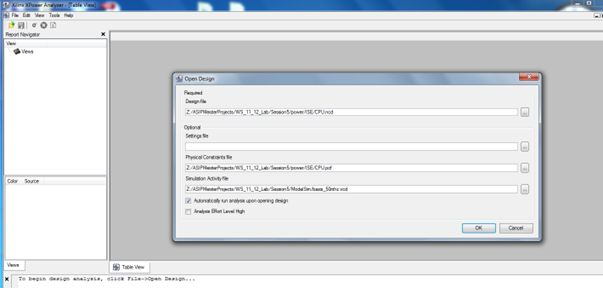
\includegraphics[width=0.9\textwidth]{src/images/7-2.png}
	\caption{Preparing xPower Tool}
	\label{fig:fig72}
\end{figure}
\emph{\textbf{Important Note:}}

It is worthy to know that the total power number that you get from
xPower is the \emph{Dynamic} power plus the \emph{Leakage} power. When
you read the leakage power consumption, you will see that is much higher
than the dynamic power. This is because the leakage power is total
leakage power consumed in the whole FPGA chip even if your design is
small and it occupies a very small part of the chip. Since Vitrex5 does
not have a power gating, the leakage power is always consumed and high.

For that, when you take the power number for your design, you have to
consider only the dynamic power in order to make your results comparable
and see clearly how much you have to pay for your custom instructions in
terms of power.
\begin{figure}[!htb]
	\centering
	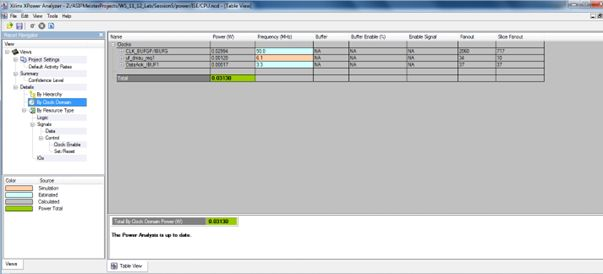
\includegraphics[width=0.9\textwidth]{src/images/7-3.png}
	\caption{Checking the CPU Frequency}
	\label{fig:fig73}
\end{figure}
To compare the power consumption between two processors, the average
value will not give correct information because every processor can
execute the same application with different execution time, as shown in Figure \ref{fig:fig73}. In this case, we need to consider
the energy. The energy is defined as the power consumed during whole
execution time, and given as:

E = P \textsubscript{*} T
\begin{figure}[!htb]
	\centering
	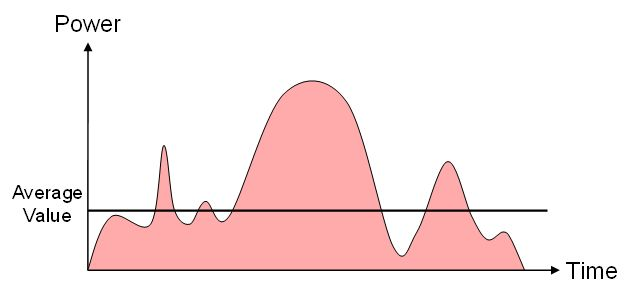
\includegraphics[width=0.9\textwidth]{src/images/7-4.png}
	\caption{Power Dissipation as Average Value}
	\label{fig:fig74}
\end{figure}
\begin{figure}[!htb]
	\centering
	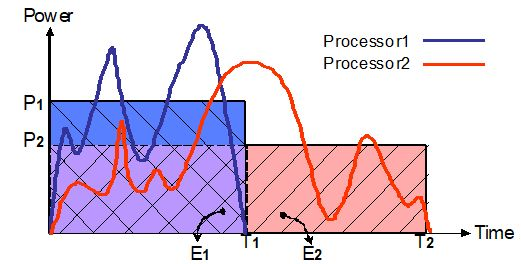
\includegraphics[width=0.9\textwidth]{src/images/7-5.png}
	\caption{Energy Comparison between two Processors}
	\label{fig:fig75}
\end{figure}
